\chapter{Multiple Importance Sampling}
\label{ch:mis}

\todo{Match to actual structure of this chapter}
In this chapter the fundamentals of Monte Carlo integration and importance sampling will be introduced.
Following that Multiple Importance Sampling is explained which is essential for the next chapter \ref{ch:mis_compensation}.


\section{Probability Basics}
\label{sec:probability_basics}
For our use case we need to define random variables, probability distribution functions (pdf) and cumulative distribution functions (cdf).
A random variable maps an event to a real number $ X: \Omega \to \mathbb{R} $.
In a discrete scenario our random variable corresponds to one exact event e.g. a dice throw showing three pips on the top.
The probability for this can be expressed as $ P(X = 3) = \frac{1}{6} $ or as $ X(3) = \frac{1}{6} $
since the random variable $ X $ can take six different values which are all equally likely.
To express the probability that an event is within a range of values we can use the cdf
which is defined as $$ F(x) = P(X \leq x), x \in \mathbb{R}. $$
For the probability of a random variable in an interval $ [a, b) $ we can write $$ P(a \leq X < b) = F(b) - F(a)~\cite{pris}. $$

When we are talking about continuous events e.g. turning a wheel of fortune, every exact angle has a probability of nearing zero.
But we can still express our probability for an angle interval with the cdf from above.
In the continuous case we have a pdf that is used to calculate the cdf with $$ F(x) = \int_{-\infty}^x p(\tilde{x}) d\tilde{x}. $$
The pdf has to be non-negative ($ \forall x: p(x) \geq 0 $) and integrate to one ($ \int_{-\infty}^{\infty} p(x) dx = 1$) to be valid and
\enquote{[...] describes the relative probability of a random variable taking on a particular value}~\cite[Chapter~13.1]{pbr-book}.
\todo{How to cite when the content of this section was created with a reference?}


\section{Generating Samples after a specific Function}
\label{sec:sample_generation}
This will be essential for the next section \ref{sec:monte_carlo},
since this is our adjustment wheel to manipulate the quality of our rendering (for a given amount of time).
Most of the time we don't need evenly distributed samples,
rather our samples should follow a specific characteristic of a material or a scene.
For this we need to know how to generate samples that correspond to that characteristic.

Given a function $ f(x) $ from which we would like to draw samples from the first step is to make sure
it fulfills the constraints for a pdf in an interval $ [a, b) $ we want to use.
First we check that $ \forall x \in [a, b): f(x) \geq 0 $ and then calculate the integral with
\begin{equation}
\label{eq:integral_fx}
    F = \int_{a}^b f(x) dx.
\end{equation}
$ F $ can be used to normalize our goal function which yields us $ \tilde{f}(x) = \frac{f(x)}{F} $ as a valid pdf.
The next step is to calculate our cdf as $ F(x) = \int_{a}^x \tilde{f}(t) dt $ which we will then invert to get $ F^{-1}(x) $.
Now we only need to draw an equally distributed random number (which most programming languages have a library for) in the interval $ [0, 1) $
which we call $ \xi $ and evaluate $ F^{-1}(\xi) = X $ to get $ X $ which is distributed proportional to $ f(.) $.
This method is called "inverse cdf"~\cite{pris}.
\todo{Should I also cover 2D sampling?}
\todo{Should I cover more sampling methods (rejection sampling e.g.)}


\section{Monte Carlo Integration}
\label{sec:monte_carlo}
Monte Carlo integration is a technique to approximate the integral of an arbitrary function $ f(x) $
by taking $ N $ random samples $ X_i $ from a pdf $ p(X_i) $.
As we know the expectation of a random variable is calculated by $$ E(X) = \int_{-\infty}^\infty x p(x) dx $$
or more generally $$ E(g(x)) = \int_{-\infty}^\infty g(x) p(x) dx. $$
For the next step we need the law of large numbers which states that $$ P\left[ \lim_{N\to\infty} \frac{1}{N} \sum_{i = 1}^N X_i = E(X) \right] = 1 $$
with $ X_i $ drawn from $ p(.) $ which means that the average of our samples will converge to the expected value~\cite[Chapter~2.4.1]{veach-thesis}.
From here we can formulate
\begin{equation*}
    \int_{a}^b g(x) p(x) dx \stackrel{definition}{=} E(g(x))
    \stackrel{law~of~large~numbers}{\approx} \frac{1}{N} \sum_{i = 1}^N g(x_i)
\end{equation*}
and with $ g(x) = \frac{f(x)}{p(x)} $
\begin{equation}
\label{eq:monte_carlo_integral}
\begin{aligned}
    \int_{a}^b \frac{f(x)}{p(x)} p(x) dx &\approx \frac{1}{N} \sum_{i = 1}^N \frac{f(x)}{p(x)} \\
    \Leftrightarrow \int_{a}^b f(x) dx &\approx \frac{1}{N} \sum_{i = 1}^N \frac{f(x)}{p(x)}
\end{aligned}
\end{equation}
which is the Monte Carlo estimator~\cite{pris}.


\subsection{Variance}
\label{sec:variance}
Generally the variance is described by $$ V(X) = \frac{1}{N} \sum_{i = 1}^N (x_i - E(X))^2 $$ for discrete random variables~\cite{pris}
and $$ V(X) = \int_{a}^b (x - I)^2 p(x) dx $$ with $ I $ being the mean of the random variable $ X $ for continuous variables~\cite{wyzant}.
When we look at the variance of our Monte Carlo integral we get
\begin{equation}
\label{eq:monte_carlo_variance}
\begin{aligned}
    V(g(x)) &= \int_{a}^b (g(x) - F)^2 p(x) dx \\
            &= \int_{a}^b \left(\frac{f(x)}{p(x)} - F\right)^2 p(x) dx
\end{aligned}
\end{equation}
with $ F $ being the integral from equation \ref{eq:integral_fx}.


\section{Importance Sampling}
\label{sec:importance_sampling}
With the variance from equation \ref{eq:monte_carlo_variance} let's see how we can improve it.
We can easily see that reducing the term $ \frac{f(x)}{p(x)} - F $ will finally reduce the variance the most since it will be exponentiated.
Since $ F $ and $ f(.) $ are fixed (that is the integral we want to calculate) only $ p(.) $ is left for modification.
When we choose $$ p(x) = \frac{f(x)}{\int_{a}^b f(x) dx} $$ we get
\begin{equation*}
\begin{aligned}
    \frac{f(x)}{p(x)} - F &= \frac{f(x)}{f(x)}\int_{a}^b f(x) dx - F \\
        &\stackrel{\ref{eq:integral_fx}}{=} \int_{a}^b f(x) dx - \int_{a}^b f(x) dx
        &= 0
\end{aligned}
\end{equation*}
which is ideal as we get a variance of 0 and are done.
The problem is that we don't know the integral at the start since that is what we want to calculate in the first place.
When we look at our chosen pdf we see that $ p(.) $ is proportional to $ f(.) $ by a factor $ \frac{1}{\int_{a}^b f(x) dx} = \frac{1}{F} := c $.
So we should at least try to chose $ p(.) $ somewhat proportional to $ f(.) $.
The difficulty is that $ f(.) $ can be arbitrary complex so we might only be able to approximate some part of it with one specific pdf.


\section{Multiple Importance Sampling}
\label{sec:multiple_importance_sampling}
The rendering equation
\begin{equation}
    \label{eq:rendering_equation}
    L_o(x, \omega) = L_e(x, \omega) + \int_{\Omega^+} f_s(x, \omega, \omega_o) L_r(x, \omega_o) |n \cdot \omega_o|^+ d\omega_o
\end{equation}
consists of the emitted light at point $ x $ $ L_e(.) $,
the bidirectional scattering distribution function (BSDF) $ f_s(.) $,
the reflected light at point $ x $ in direction $ \omega $ expressed as $ L_r(.) $
and the cosine to account for looking at an angle onto the surface $ |n \cdot \omega_o|^+ $
where the $ ^+ $ means we are only taking values $ > 0 $ so only directions pointing into the upper hemisphere.
With this we can see that a single pdf that only is proportional to e.g., the BSDF leaves out the $ L_r(.) $ term so it can't be optimal.
Having multiple pdfs where each samples a different part of the rendering equation well
a combination of them should create a good result.
E. Veach created a good example of this problem in his thesis~\cite{veach-thesis} which can be seen in figure \ref{fig:veach_mis_single}.
He also introduced Multiple Importance Sampling to use a combination of pdfs to get better results than would be possible with only one pdf.

When sampling only the BSDF we see that in figure \ref{fig:veach_mis_bsdf} the bottom left reflection is very noisy,
because sampling a diffuse BSDF can give a wide range of directions
and since the light source on the left is very small only very few directions will point directly on that light source.
The more specular surfaces in that figure are well sampled which makes sense,
because there are less possible directions to sample so the reflection will be well sampled.

On the other hand figure \ref{fig:veach_mis_light} shows the same scene but sampled after the light sources
by sampling a random point on the light source and then evaluating the render equation to get the contribution.
Here the opposite happened in the two corners we looked at before.
The bottom left reflection is very well sampled
since the direction to the light source is still valid (has some contribution in the BSDF) and therefore we can see the whole reflection.
But now the top right reflection is noisy because the direction to a random point on the light source has no contribution in the BSDF.

\begin{figure}
    \centering
    \begin{subfigure}[b]{0.45\textwidth}
        \centering
        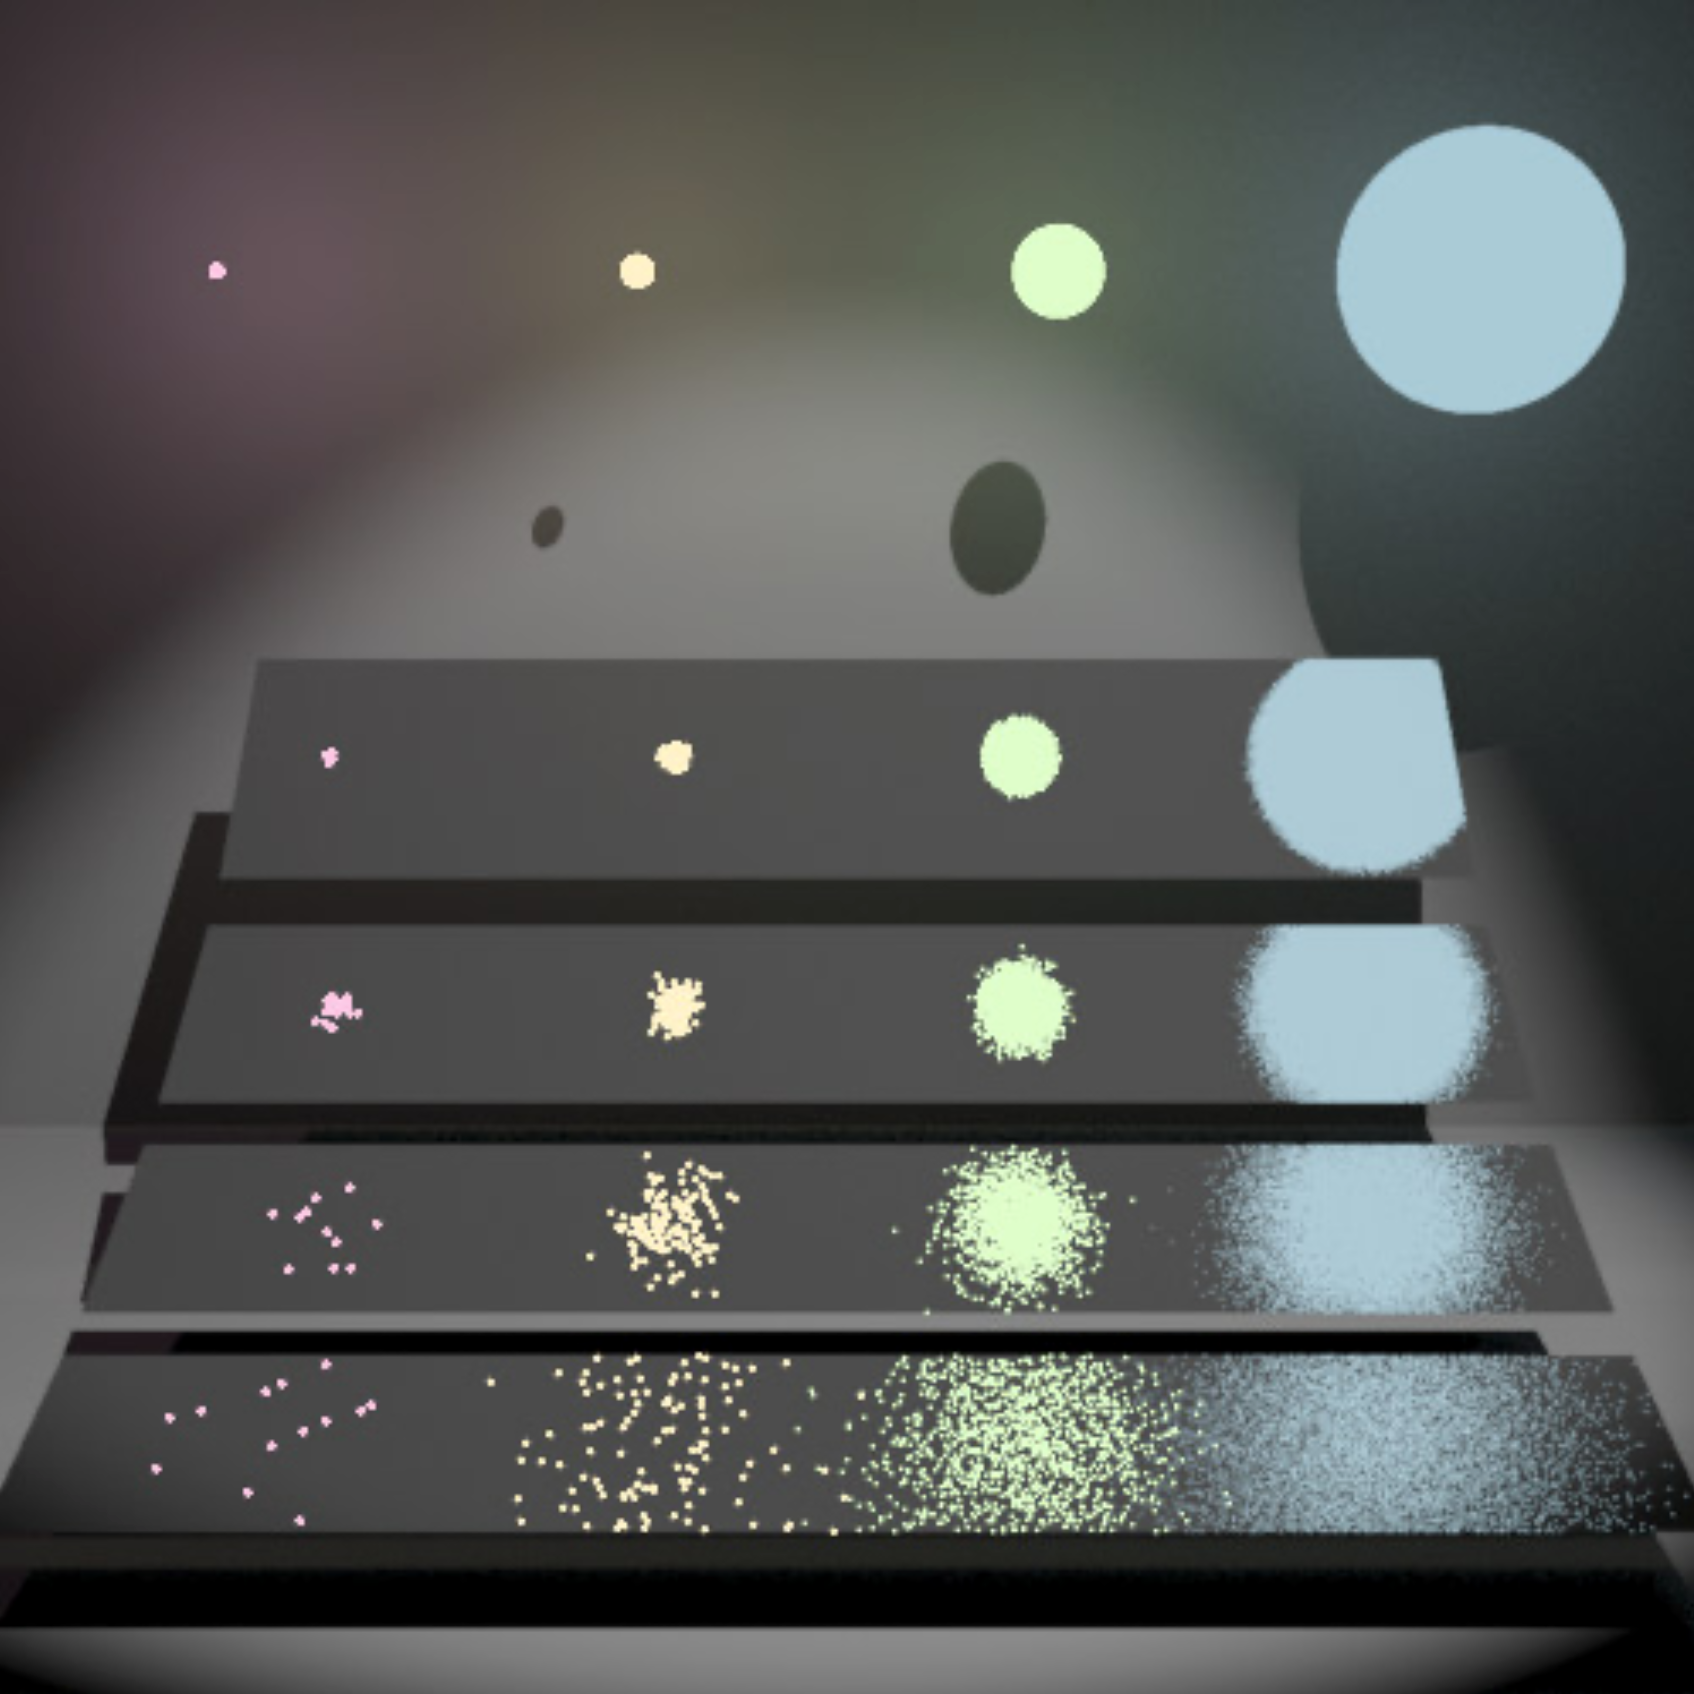
\includegraphics[width=\textwidth]{images/veach_mis_bsdf.png}
        \caption{Sampled after the BSDF}
        \label{fig:veach_mis_bsdf}
    \end{subfigure}
    \hfill
    \begin{subfigure}[b]{0.45\textwidth}
        \centering
        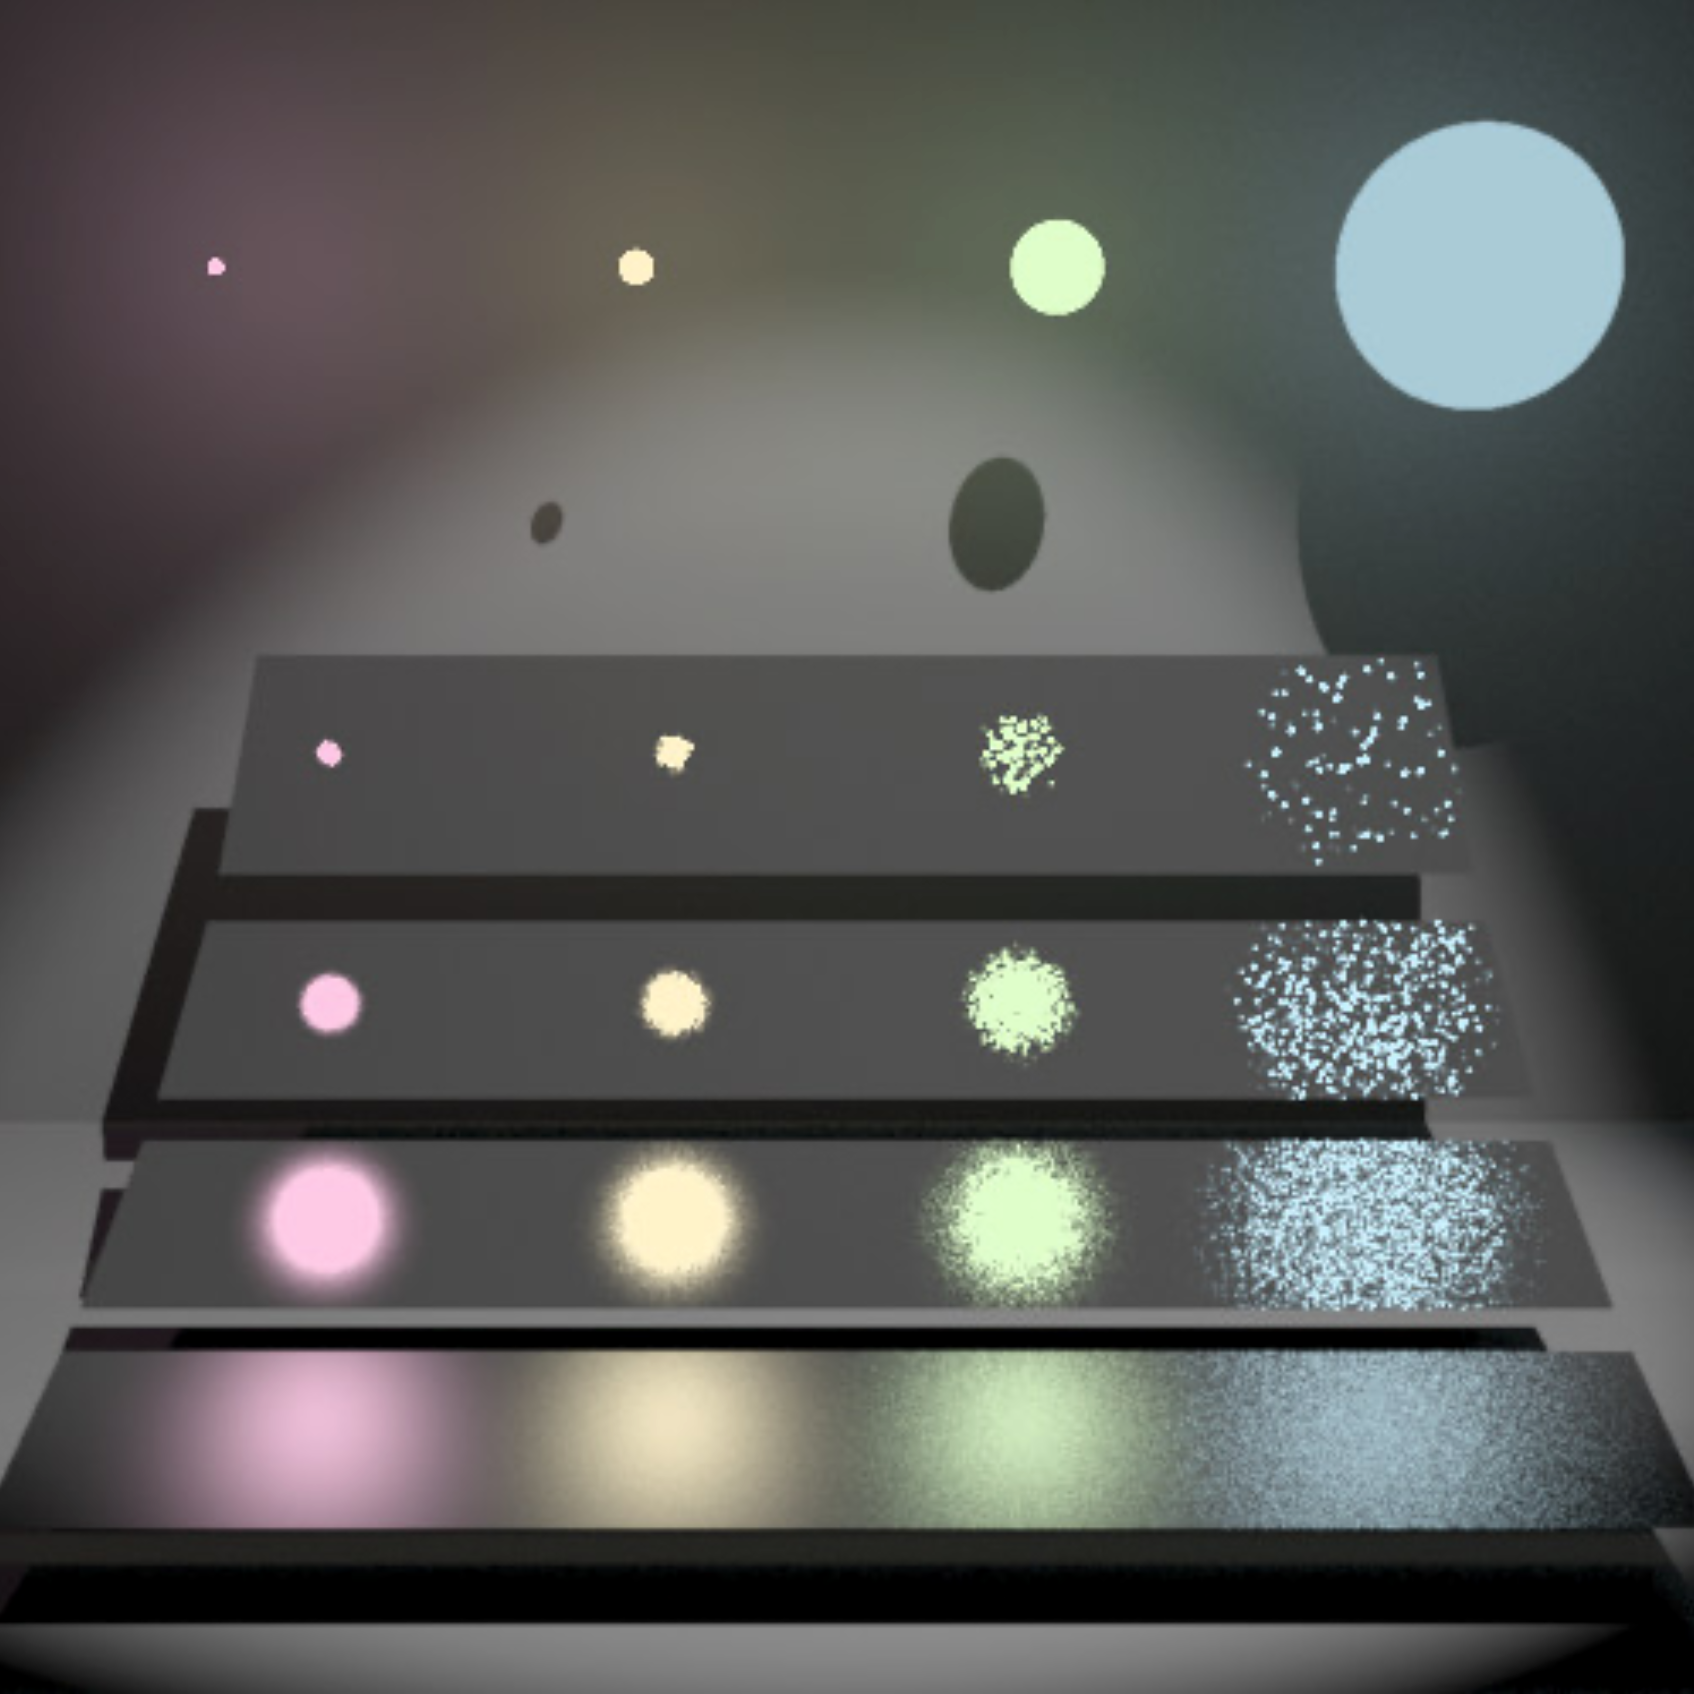
\includegraphics[width=\textwidth]{images/veach_mis_light.png}
        \caption{Sampled after the light sources}
        \label{fig:veach_mis_light}
    \end{subfigure}
    \caption{A scene with four light sources getting larger in diameter from left to right
    and four horizontal objects with BSDFs from diffuse at the bottom to more and more specular at the top.\\
    (a) This scene is sampled using a pdf that is proportional to the BSDF of the surface.\\
    (b) Here the scene was sampled with a pdf that generated samples on the light source.
    These graphics were taken from~\cite[Figure~9.2]{veach-thesis}.}
    \label{fig:veach_mis_single}
\end{figure}

If we could combine both approaches the result should cover all cases and show all reflections well.
To do this Veach introduced Multiple Importance Sampling~\cite[Chapter~9]{veach-thesis}.
The updated estimator now looks like this: $$ F = \sum_{i = 1}^k \frac{1}{n_i} \sum_{j = 1}^{n_i} w_i(X_{i,j}) \frac{f(X_{i,j})}{p(X_{i,j})}. $$
Compared to the initial estimator from equation \ref{eq:monte_carlo_integral} we now have additional weight functions $ w_i(.) $
and split up our samples over the $ k $ different sampling technique with $ n = \sum_{i = 1}^k~n_i $.
To keep the estimator unbiased the weighting function need to fulfill two constraints:
\begin{itemize}
    \item $ \sum_{i = 1}^n w_i(x) = 1 $ when $ f(x) \neq 0 $
    \item $ w_i(x) = 0 $ when $ p_i(x) = 0 $.
\end{itemize}
The first constraint makes sure that every point is neither reduced nor increased in its contribution
which is important to keep the estimator unbiased.
The second constraint states that a pdf that could not create this sample also must have no weight
so it will be ignored.
A concrete weighting function will be introduced in the next subsection.


\subsection{Balance Heuristic}
\label{sec:balance_heuristic}
A very popular weighting function also introduced by Veach is the balance heuristic~\cite[Chapter~9.2.2]{veach-thesis}.
The formula to calculate it is as follows: $$ w_i(x) = \frac{n_i p_i(x)}{\sum_{j = 1}^k n_j p_j(x)} $$
So the weight for a sample consists of the amount of samples $ n_i $ drawn with that technique,
the probability $ p_i(x) $ for that sample divided by the sum of all techniques.
\todo{show how it falls down to a simple standard monte carlo estimator when inserting into the formula (when more text is needed?)}

\begin{figure}[h]
    \centering
    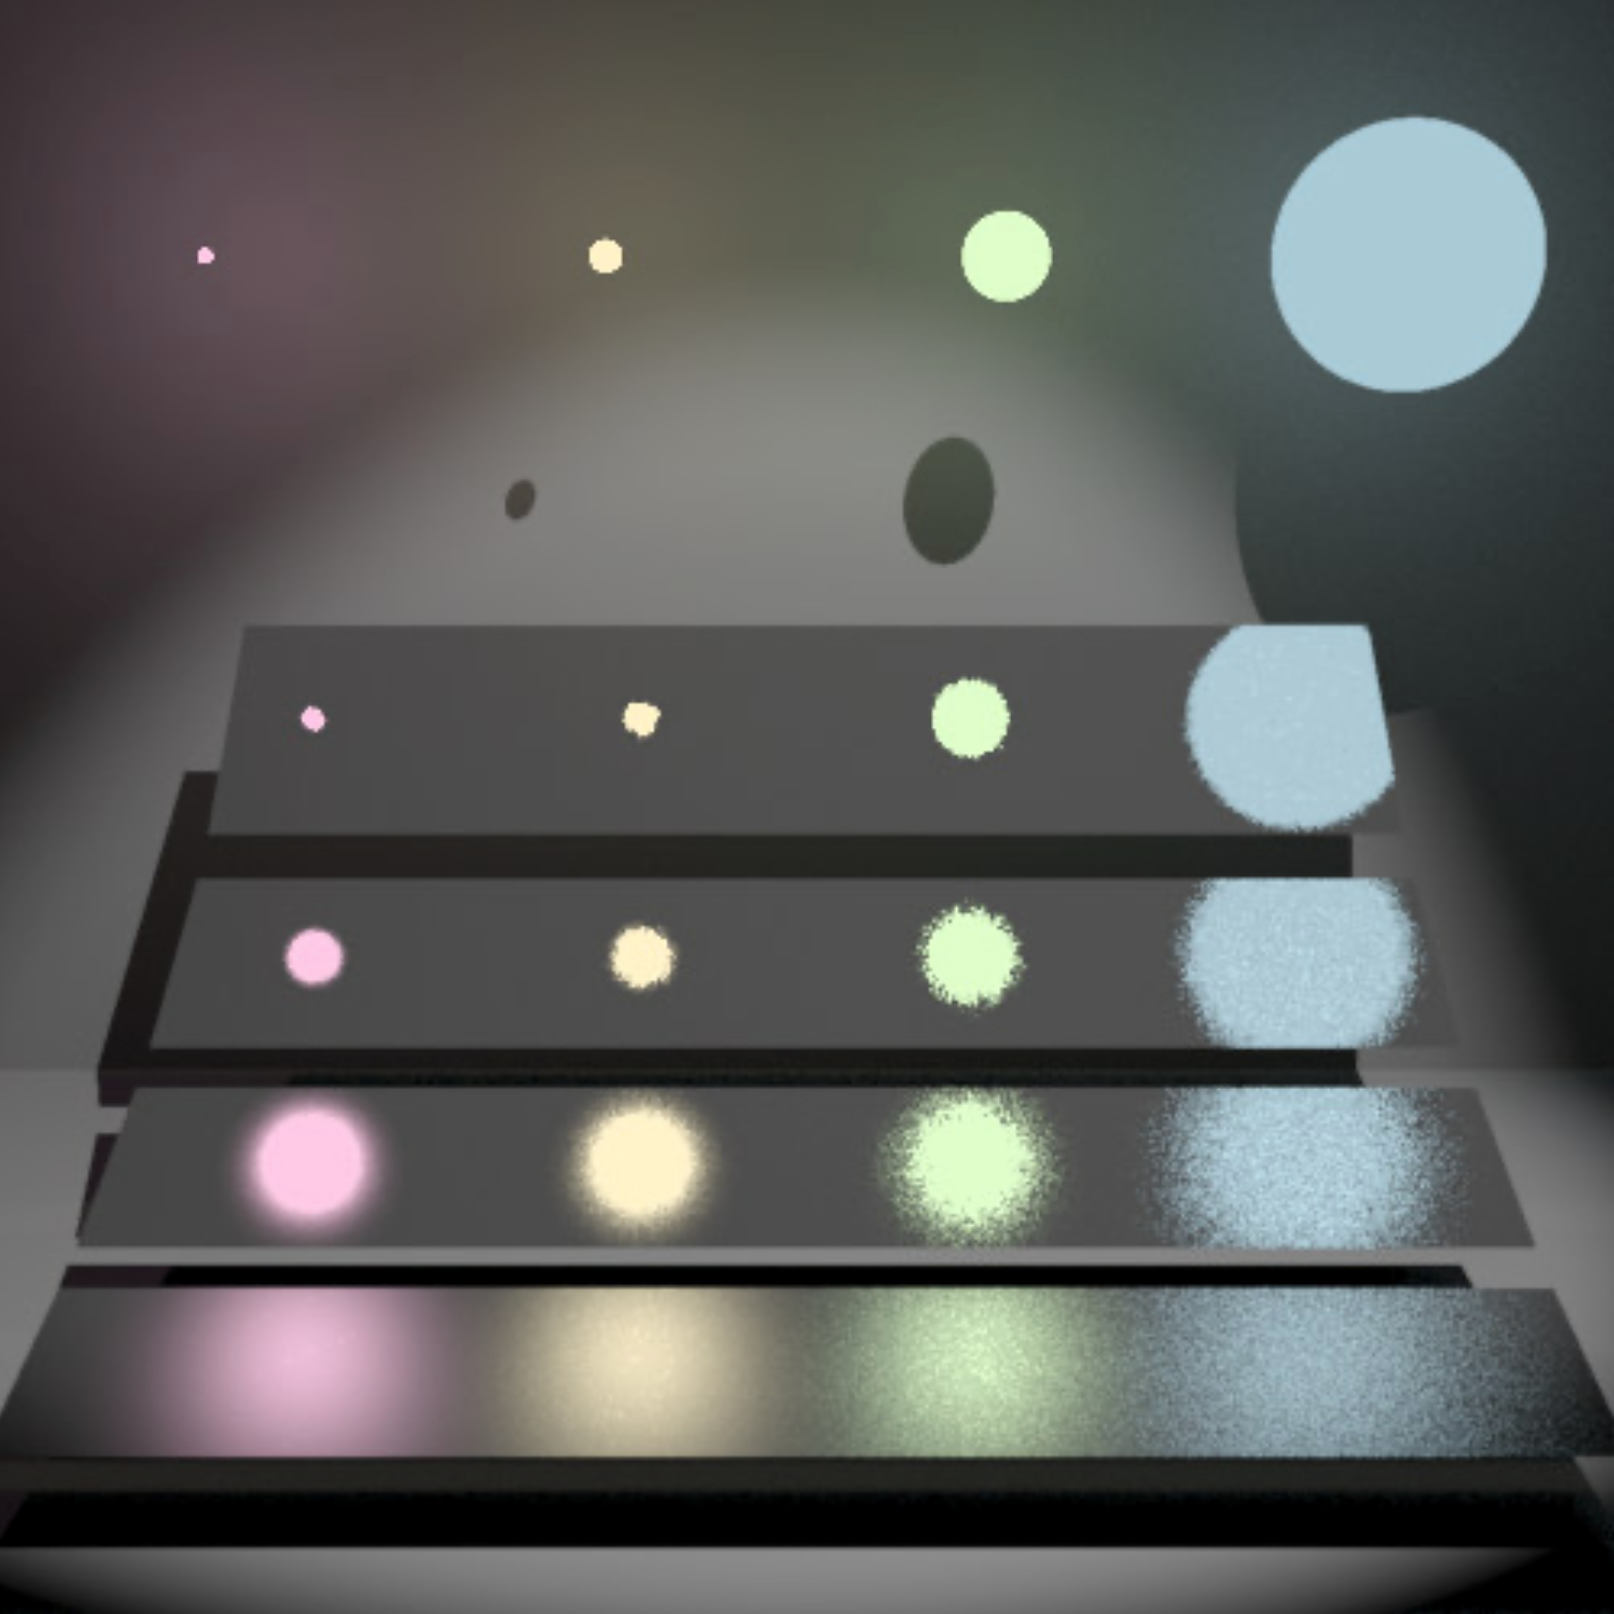
\includegraphics[width=.45\textwidth]{images/veach_mis_both.png}
    \caption{This image shows the same scene as in figure \ref{fig:veach_mis_single} but rendered using the balance heuristic. Taken from~\cite[Figure~9.4]{veach-thesis}.}
    \label{fig:veach_mis_balance}
\end{figure}

Figure \ref{fig:veach_mis_balance} show that with the balance heuristic the noisy areas we observed
while only using a single pdf in figure \ref{fig:veach_mis_single} disappeared
and all combinations of surface roughness and light source size are well represented.